\documentclass[12pt]{elsart}
\usepackage{amsmath}
\usepackage{amssymb}
\usepackage{program}
\usepackage{graphicx}
\newcommand{\field}[1]{\mathbb{#1}}
\usepackage{algorithm}
\usepackage{algpseudocode}



%%%%%%%%%%%%%%%%%%%%%%%%%%%%%%%%%%%%%%%%%Space to make more readable!
%\vspace{10 mm}
%%%%%%%%%%%%%%%%%%%%%%%%%%%%%%%%%%%%%%%%%Take out later!

\begin{document}
Bryan Burkhardt - XMV643\\
CS3343 Section 01\\
15 Oct 2017\\

\pagestyle{empty}

\begin{center}
\Large  CS3343 Analysis of Algorithms Fall 2017 \\
\large {\bf Homework 4}\\
\normalsize Due 10/15/17 before 11:59pm (Central Time)
\end{center}

{\bf 1.  Heapsort (4 points)}

Originally we stored our heap in an array.  Consider instead storing our heap as a doubly linked list.  

\begin{enumerate}
   \item (2 points) For a node $i$ what are the new asymptotic run times for  $left(i)$, $right(i)$, and $parent(i)$?  Justify your answer.
$\bf{Answers:}$
	\begin{enumerate}
	\item $left(i)$ is $O(i)$ because the node locations in memory are unknown since it's a linked list. This restricts us from being able to jump straight to the left child.
	\item $right(i)$ is $O(i)$ for the same reason $left(i)$ is $O(i)$
	\item $parent(i)$ is $O(i/2)$ because we know the parent will come before the children in the linked list. However, $O(i/2)$ is still $O(i)$\\
	\end{enumerate}

  \item (2 points) How does this affect the run times of findMax(), insert(key), extractMax()?  Justify your answer.\\
	$\bf{Answers:}$
	\begin{enumerate}
	\item findMAX() is $O(1)$ because it will always be the head node of our doubly linked list. In a linked list, the head node is always known.
	\item insert(key) is $O(i^2)$ because we first have to insert the new key at the end of the linked list which will take $i$ operations. Then we must heapify which will take another $i^2$ times going through it to reorder all the nodes.
	\item extractMAX() is $O(i^2)$ Because we must traverse to the last element, swap it with the head node which is $i+1$ times, then heapify which will require $i^2$ operations.
	\end{enumerate}
\end{enumerate}
\newpage
{\bf 2.  Counting Sort (4 points)}

\begin{algorithm}
\caption{void countingSort(int $A[1\ldots n]$, int $k$)}
 \begin{algorithmic}[1]
 \State //Precondition: The $n$ values in $A$ are all between $0$ and $k$
 \State Let $C[0\ldots k]$ be a new array
 \State //We will store our sorted array in the array $B$.
 \State Let $B[1\ldots n]$ be a new array 
\For{$i = 0$ {\bf to} $k$}
        \State $C[i]=0$;
  \EndFor
\For{$i = 1$ {\bf to} $n$}
        \State $C[A[i]]=C[A[i]]+1$;
  \EndFor
\State //$C[i]$ now contains the \# of elements in $A$ equal to $i$
\For{$i = 1$ {\bf to} $k$}
        \State $C[i]=C[i]+C[i-1]$;
  \EndFor
\State //$C[i]$ now contains the \# of elements in $A$ that are $\leq$ to $i$
\For{$i = n$ {\bf down to} $1$}
        \State $B[C[A[i]]]=A[i]$;
        \State $C[A[i]]=C[A[i]]-1$;
  \EndFor
\State return $B$;
\end{algorithmic}
\end{algorithm}

\begin{enumerate}
   \item (2 points) Illustrate the operation of $countingSort(\{2,1,5,3,1,2,5\},6)$.  Specifically, show the changes made to the arrays $A$, $B$, and $C$ for each pass through the for loop at line 16.\\
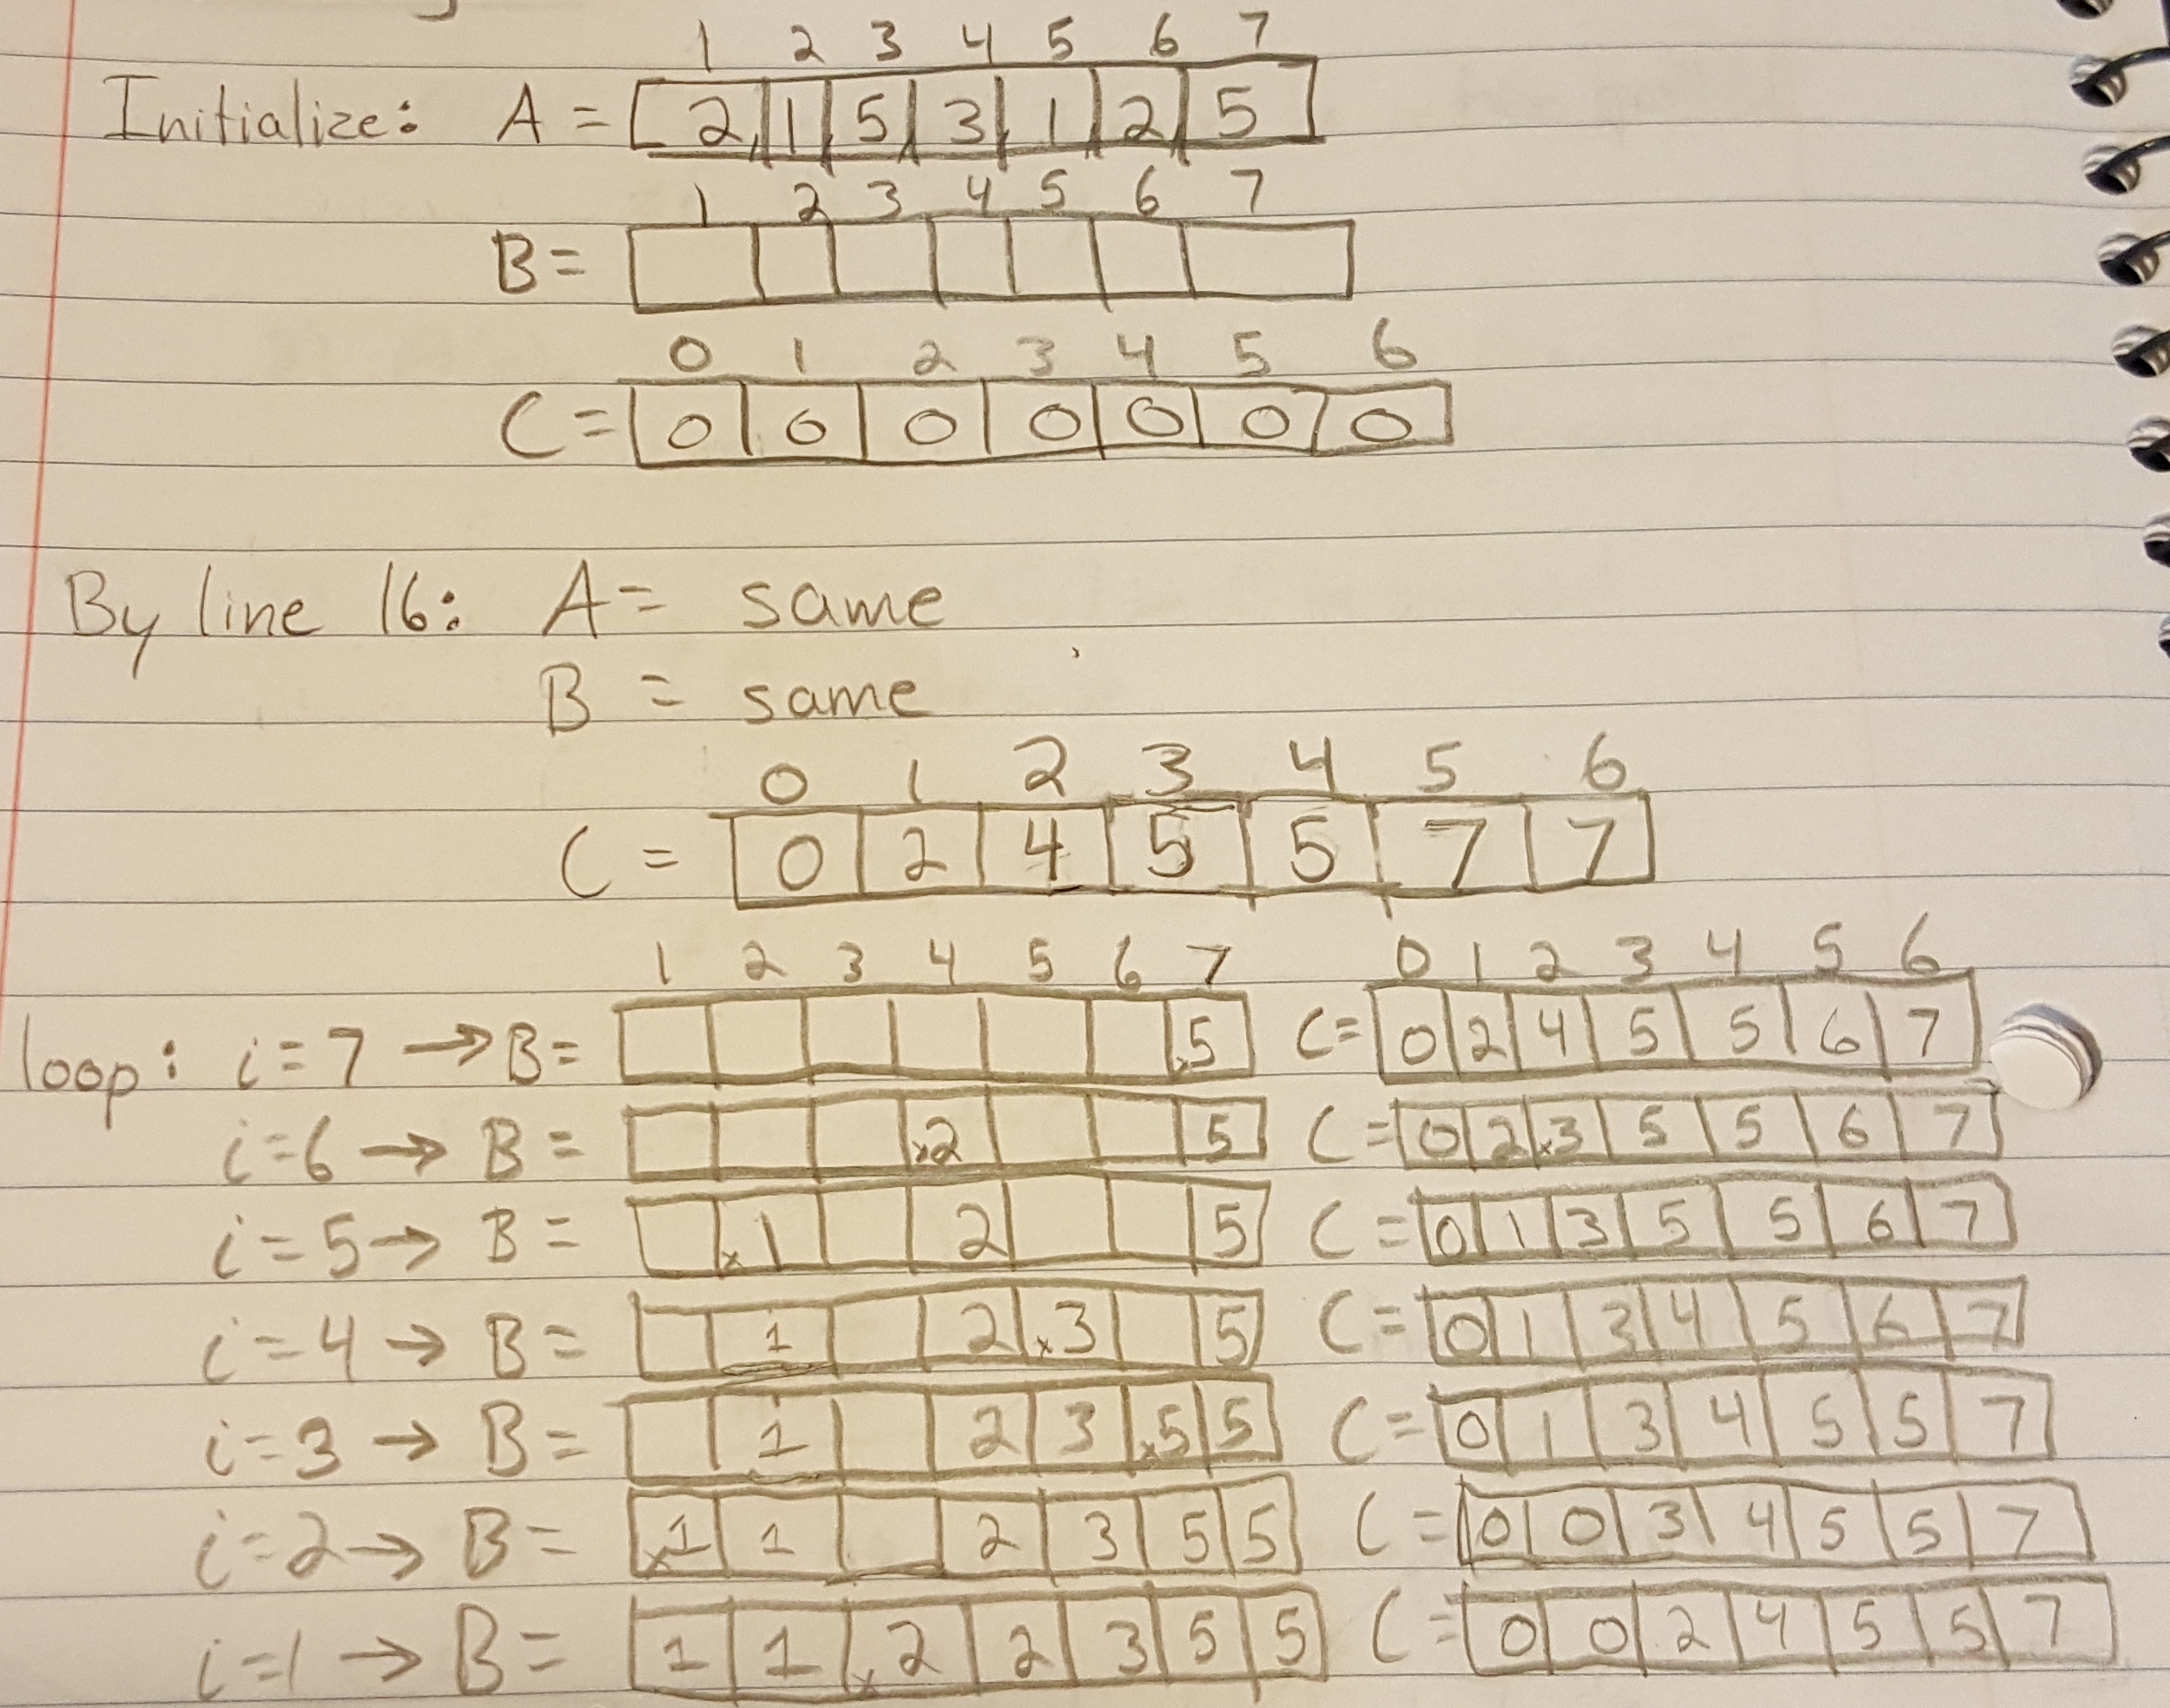
\includegraphics[scale=0.12]{countingSortArrays.jpg}
\newpage

   \item (2 points) Describe an algorithm that, given an unsorted array of $n$ integers in the range $0$ to $k$, preprocesses its
input and then answers any query about how many of the $n$ integers fall into a range $a$ to $b$ in $O(1)$ time. Your algorithm should use $O(n+k)$ preprocessing time.
\\\\(Hint: Look at the array $C$ which is computed by the above code for inspiration)\\\\
$\bf{Answer:}$ By line 15 of the algoritm, the preprocessing time is at $O(n+k)$ which was given by the profesor. Also, at this point in the algorithm, the array $C=[0,2,4,5,5,7,7]$. By looking at this array, we can see the values at each $C[i]$ indicate how many numbers in the unsorted array are $\leq i$. Therefore, if we wanted to know how many integers are in the range between $a$ and $b$ in $O(1)$ time, we simply do:
\begin{algorithmic}
\If{(a==0)}
	\State return C[b];
\Else
	\State return C[b] $-$ C[a$-$1];
\EndIf
\end{algorithmic}
\end{enumerate}
{\bf 3.  Hash Table (7 points)}

\begin{enumerate}
   \item Consider inserting the keys $2, 21, 3, 58, 11, 42, 34$ into a hash
table of length $m = 10$ with the hash function $h(k) = k \bmod 10$.
\begin{enumerate}
   \item (2 points)  Illustrate the result of inserting these keys using linear probing to resolve collisions.\\
	\begin{tabular}{|c|c|}
		\hline
		${\bf Index}$ & ${\bf Key}$\\
		\noalign{\hrule height 1pt}
		0 & NULL\\
		\noalign{\hrule height .5pt}
		1 & 21\\
		\noalign{\hrule height 1pt}
		2 & 2\\
		\noalign{\hrule height 1pt}	
		3 & 3\\
		\noalign{\hrule height 1pt}		
		4 & 11\\
		\noalign{\hrule height .5pt}
		5 & 42\\
		\noalign{\hrule height .5pt}
		6 & 34\\
		\noalign{\hrule height .5pt}
		7 & NULL\\
		\noalign{\hrule height 1pt}
		8 & 58\\
		\noalign{\hrule height 1pt}
		9 & NULL\\
		\hline
	\end{tabular}
\newpage
   \item (2 points) Illustrate the result of inserting these keys using chaining to resolve collisions.\\
	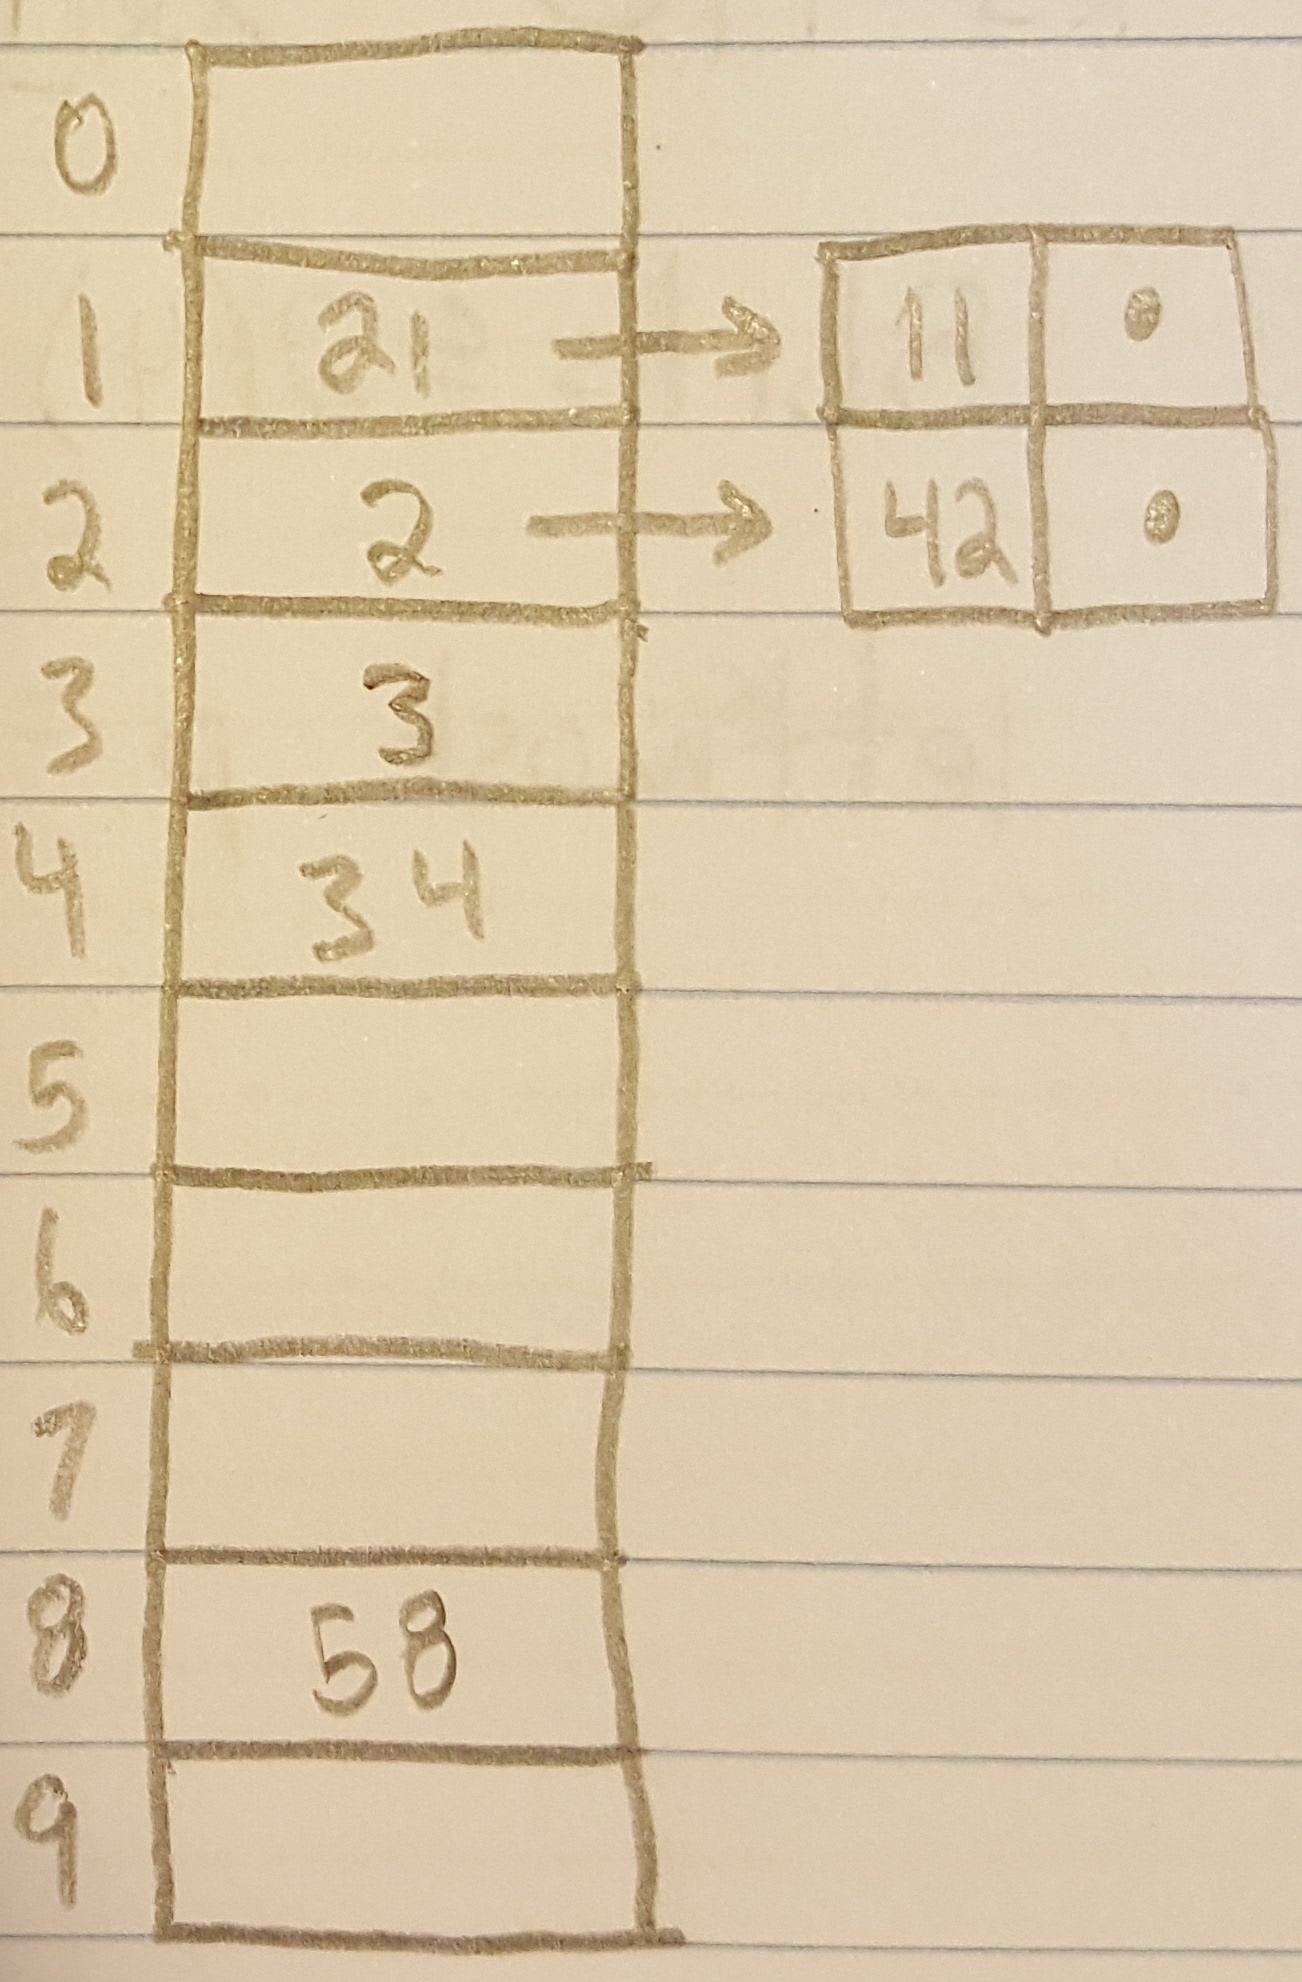
\includegraphics[scale=0.12]{3-1-b.jpg}
\end{enumerate}

   \item Consider inserting the keys $8,5,14$ into a hash
table of length $m = 8$ with the hash function $h(k) = \lfloor m(kA - \lfloor kA\rfloor)\rfloor$ where $A=0.625$.
\begin{enumerate}
   \item (2 points) Illustrate the result of inserting these keys.\\
	\begin{tabular}{|c|c|}
		\hline
		${\bf Index}$ & ${\bf Key}$\\
		\noalign{\hrule height 1pt}
		0 & 8\\
		\noalign{\hrule height .5pt}
		1 & 5\\
		\noalign{\hrule height 1pt}
		2 & NULL\\
		\noalign{\hrule height 1pt}	
		3 & NULL\\
		\noalign{\hrule height 1pt}		
		4 & NULL\\
		\noalign{\hrule height .5pt}
		5 & NULL\\
		\noalign{\hrule height .5pt}
		6 & 14\\
		\noalign{\hrule height .5pt}
		7 & NULL\\
		\hline
	\end{tabular}
\newpage
   \item (1 point) Now compute the hash function of the key $14$ using the implementation we described in our notes.  
\\\\You can assume we have a word size $w=4$. Since $m=8=2^3$, $p=3$.  Since $A=0.625=10/2^4=10/2^w$, $s=10$.
\\\\(Hint: Compute $ks$ and convert it to a binary number.  This number will consist of $\leq 2w$ bits.  Look at the rightmost $w$ bits.  Of those bits, convert the leftmost $p$ bits back to an integer.  This integer is your hash table slot.)\\\\
	{\bf Answer:}\\
	$k = 14, s = 10, w  = 4, p = 3$\\
	$ks = (14)(10) = 140$\\
	$140 = 10001100$ in binary which is $\leq 2w$ bits $\leq 2(4)$ bits $\leq 8$ bits\\
	Rightmost  $4$ bits $= 1100$\\
	Leftmost $p=3$ bits $= 110$\\
	Binary $110 = 6$ which is the correct hash table slot for key $14$\\
\end{enumerate}


\end{enumerate}

\end{document}